\newthought{\textbf{Adinda Awaliah - 2020903430004 - TRKJ 3B}}

\newday{\textbf{1-2 desember 2022} - Instalasi dan Konfigurasi Apache Hadoop}
\begin{enumerate}
\item Kendala dan Solusi
\newline praktikum instalasi apache hadoop tidak ada kendala. konfigurasi apache hadoop terkendala pada saat perintah jps, hasil yang muncul hanya 2jps, solusinya kembali ke langkah ssh, dan untuk menampilkan jps harus berada pada /usr/local/hadoop/etc/hadoop

\item Kesimpulan
\newline berhasil melakukan instalasi. berhasil melakukan konfigurasi.

\begin{figure}[!ht]
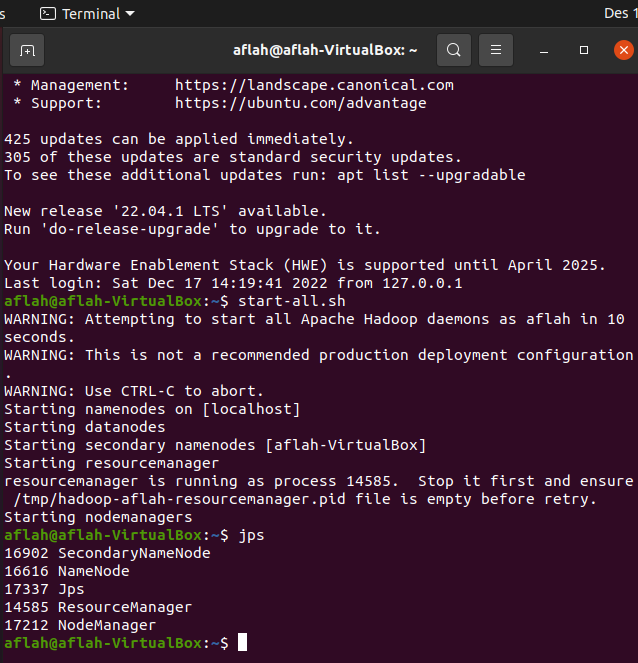
\includegraphics[width=\textwidth]{AdindaAwaliah/jps}
\caption{hasil dari jps}
\label{gam:jps}
\end{figure}

\begin{figure}
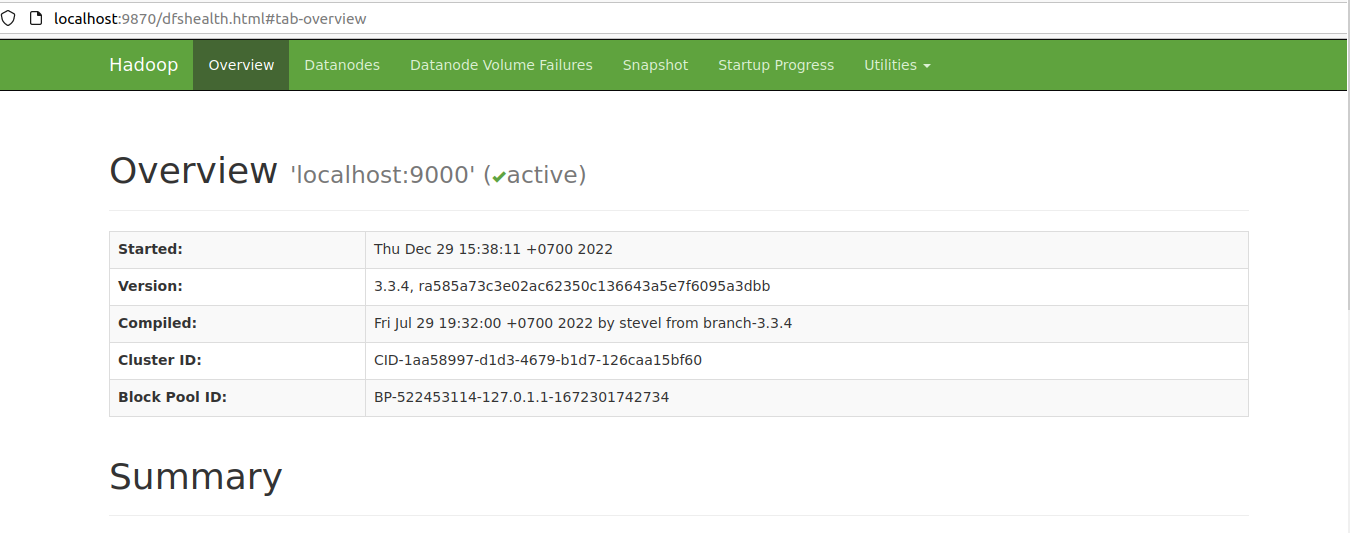
\includegraphics[width=\textwidth]{AdindaAwaliah/konfigurasi apache hadoop web 9870}
\caption{apache hadoop web 9870}
\label{gam:konfigurasi apache hadoop web 9870}
\end{figure}

\begin{figure}
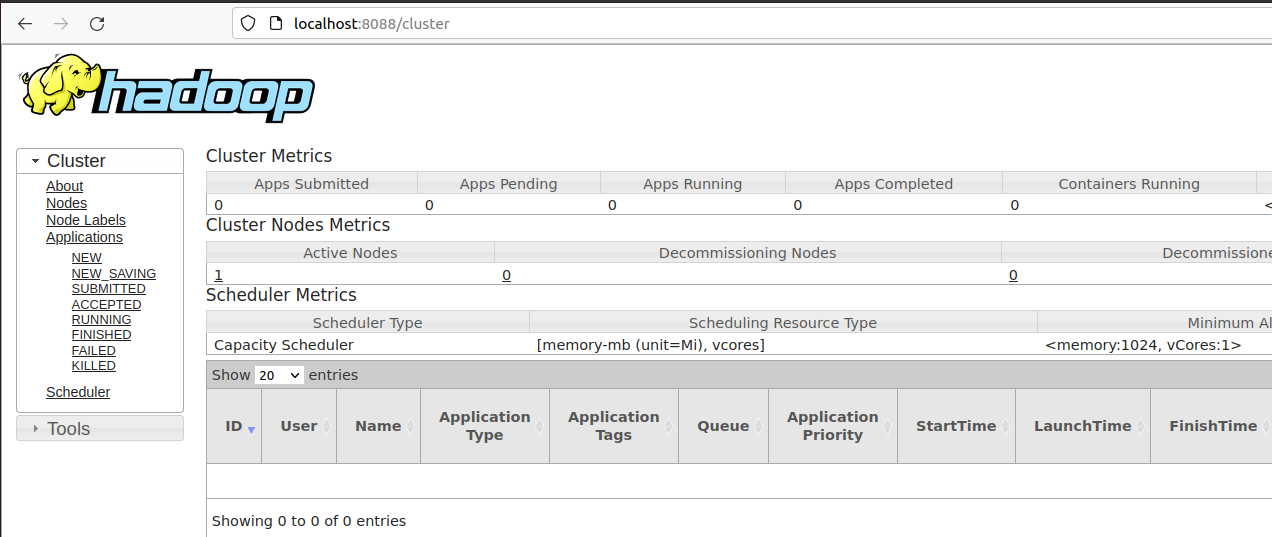
\includegraphics[width=\textwidth]{AdindaAwaliah/konfigurasi apache hadoop web 8088}
\caption{apache hadoop web 8088}
\label{gam:konfigurasi apache hadoop web 8088}
\end{figure}

\end{enumerate}

\newday{\textbf{ 8-9 desember 2022}}
\begin{enumerate}
\item Kendala dan Solusi
% jelaskan kendala dan penyebab yang dialami saat mengikuti praktikum serta solusi atau langkah-langkah yang telah dilakukan

\item Kesimpulan
% berikan kesimpulan dari praktikum yang telah dikerjkan
\newline lanjutan instalasi apache hadoop

\end{enumerate}


\newday{\textbf{15 desember 2022}- Program WordCount bawaan Hadoop}
\begin{enumerate}
\item Kendala dan Solusi
\newline Pada saat melakukan pratikum tidak ada kendala

\item Kesimpulan
\newline Berhasil melakukan praktikum WordCount bawaan Hadoop

\begin{figure}[!ht]
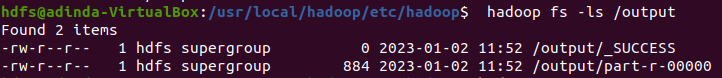
\includegraphics[width=\textwidth]{AdindaAwaliah/hasil ss no 6 wordcount}
\caption{Cek Hasil WordCount Hadoop}
\label{gam:hasil ss no 6 wordcount}
\end{figure}

\begin{figure}[!ht]
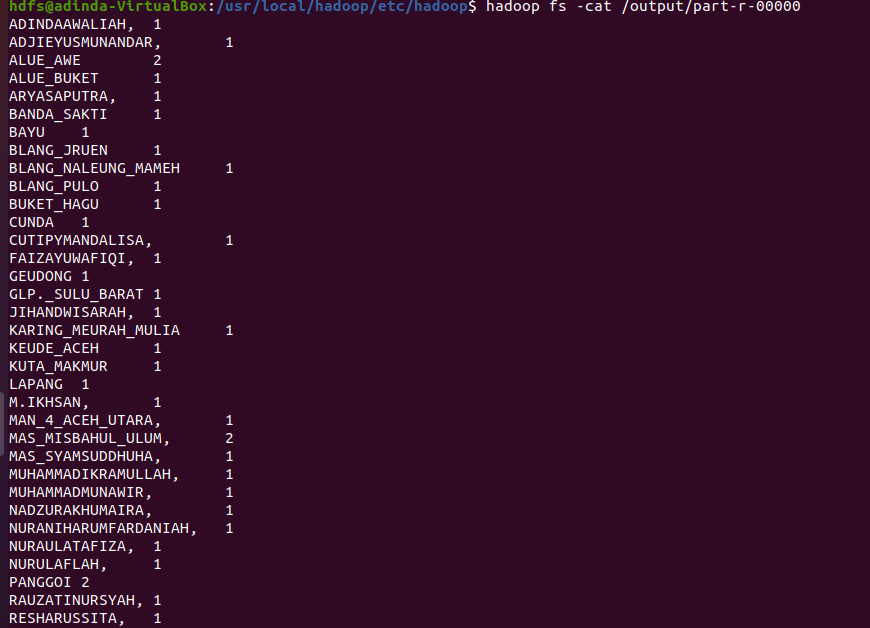
\includegraphics[width=\textwidth]{AdindaAwaliah/hasil ss no 7 wordcount}
\caption{Lihat Hasil WordCount Hadoop}
\label{gam:hasil ss no 7 wordcount}
\end{figure}

\end{enumerate}

\newday{\textbf{16 desember 2022}- Program WordCount dengan Java }
\begin{enumerate}
\item Kendala dan Solusi
\newline Tidak ada kendala saat mengerjakan praktikum

\item Kesimpulan
\newline Berhasil menampiklan hasil WordCount Java

\begin{figure}[!ht]
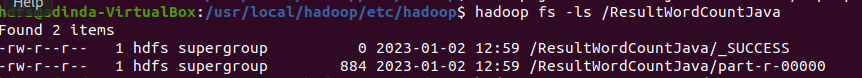
\includegraphics[width=\textwidth]{AdindaAwaliah/hasil ss no 9 wordcount java}
\caption{Cek hasil WordCount Java}
\label{gam:hasil ss no 9 wordcount java}
\end{figure}

\begin{figure}[!ht]
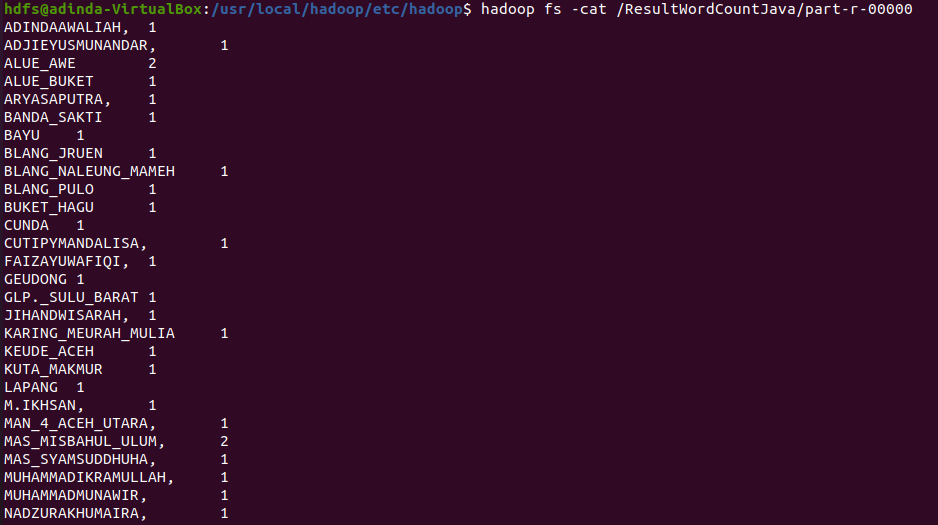
\includegraphics[width=\textwidth]{AdindaAwaliah/hasil ss no 10 wordcount java}
\caption{Lihat hasil WordCount Java}
\label{gam:hasil ss no 9 wordcount java}
\end{figure}

\end{enumerate}

\newday{\textbf{22 desember 2022}- Instalasi ApacheSpark}
\begin{enumerate}
\item Kendala dan Solusi
\newline Saat mengerjakan praktikum ini tidak ada kendala saat mengerjakan praktikum

\item Kesimpulan
\newline Berhasil melakukan installasi

\begin{figure}[!ht]
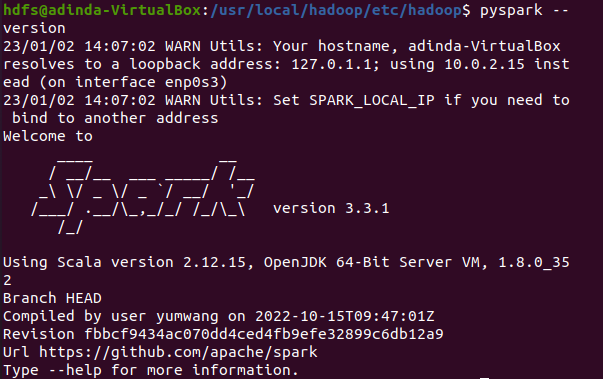
\includegraphics[width=\textwidth]{AdindaAwaliah/instalasi apache spark no 5}
\caption{Versi Spark yang terinstall}
\label{gam:instalasi apache spark no 5}
\end{figure}

\end{enumerate}

\newday{\textbf{23 desember 2022}- Program WordCount dengan Python }
\begin{enumerate}
\item Kendala dan Solusi
\newline Terkendala saat perintah menjalankan program dengan hadoop pada ~/WordCountPython/map.py -reducer tidak bisa. Solusinya  di ganti dengan /usr/local/hadoop/etc/hadoop karena sebelumnya saya sudah menjalankan program di dalam /usr/local/hadoop/etc/hadoop

\item Kesimpulan
\newline Berhasil melakukan pratikum wordcount python

\begin{figure}[!ht]
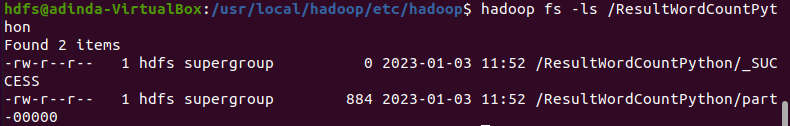
\includegraphics[width=\textwidth]{AdindaAwaliah/hasil ss no 8 wordcount python}
\caption{Cek hasil WordCount Python}
\label{gam:hasil ss no 8 wordcount python}
\end{figure}

\begin{figure}[!ht]
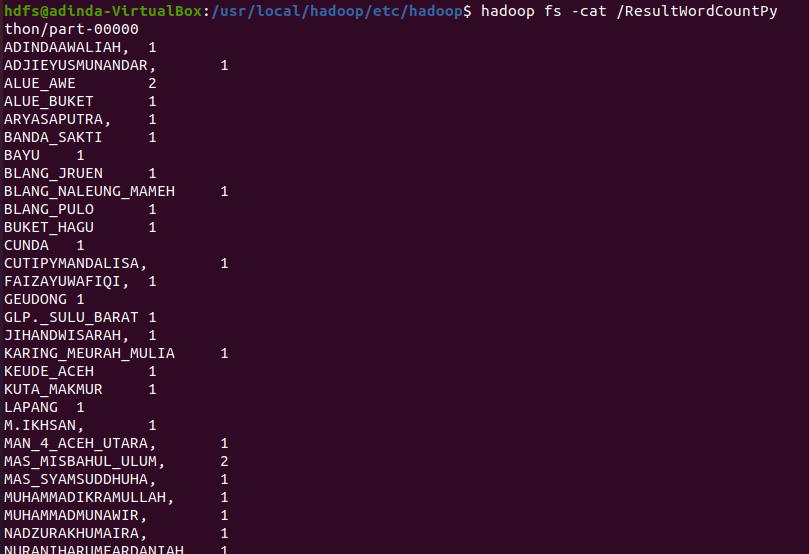
\includegraphics[width=\textwidth]{AdindaAwaliah/hasil ss no 9 wordcount python}
\caption{Lihat hasil WordCount Python}
\label{gam:hasil ss no 9 wordcount python}
\end{figure}

\end{enumerate}


\newday{\textbf{23 desember 2022}- Program WordCount dengan PySpark }
\begin{enumerate}
\item Kendala dan Solusi
\newline Saat bmengerjakan praktikum ini, tidak ditemukan kendala

\item Kesimpulan
\newline Berhasil melakukan pratikum wordcount PySpark

\begin{figure}[!ht]
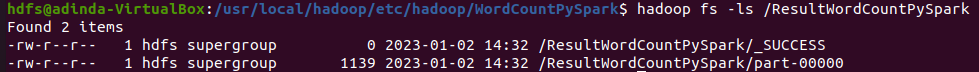
\includegraphics[width=\textwidth]{AdindaAwaliah/wordcup dengan pyspark no 6}
\caption{Cek hasil WordCount PySpark}
\label{gam:wordcup dengan pyspark no 6}
\end{figure}

\begin{figure}[!ht]
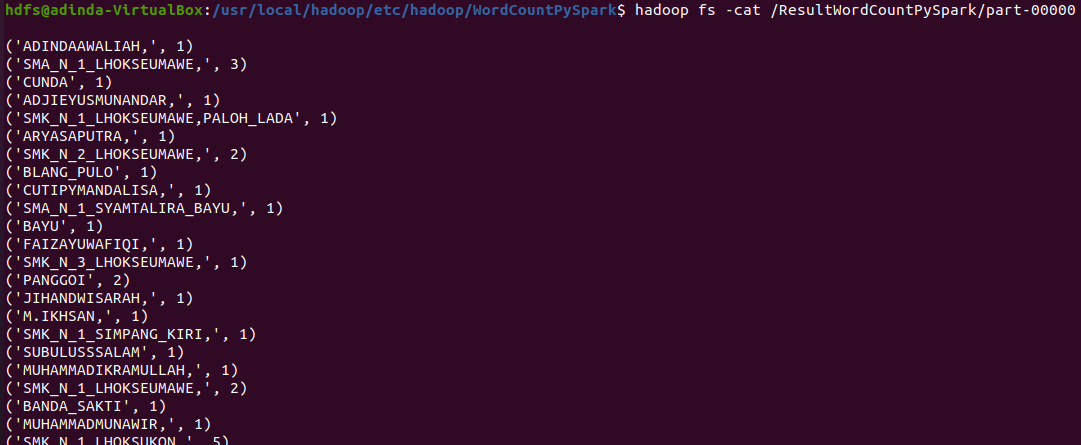
\includegraphics[width=\textwidth]{AdindaAwaliah/wordcup dengan pyspark no 7}
\caption{Lihat hasil WordCount PySprak}
\label{gam:wordcup dengan pyspark no 7}
\end{figure}

\end{enumerate}

\newday{\textbf{05 Januari 2023}- Tugas individu Program Machine Learning dengan Pyspark }
\begin{enumerate}
\item Kendala dan Solusi
\newline a. Kendala pertama pada saat menentukan nilai K 		dengan metode silhoutte, grafik tidak muncul, seharusnya setelah perintah plt.show() akan muncul grafik, belum di temukannya solusi
\newline b. Kendala selanjutnya saat menampilkan hasil Clustering dengan PCA, grafik tidak muncul, seharusnya setelah perintah plt.show() akan muncul grafik dan belum di temukannya solusi

\begin{figure}[!ht]
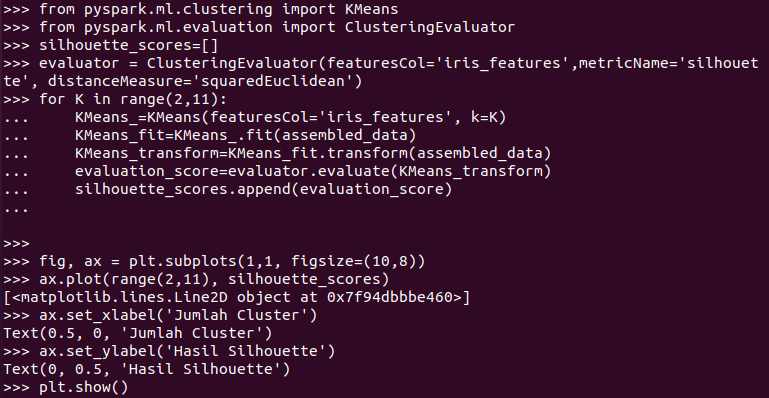
\includegraphics[width=\textwidth]{AdindaAwaliah/kendala grafik 1 nomor 5}
\caption{kendala pertama grafik tidak muncul}
\label{gam:kendala grafik 1 nomor 5}
\end{figure}


\item Kesimpulan
\newline Pada percobaan praktikum ini berhasil memunculkan tabel, namun tidak berhasil untuk memunculkan grafik. Tabel yang muncul merupakan tabel dari load data iris dan tabel penentuan nilai K asseamble data.

\begin{figure}[!ht]
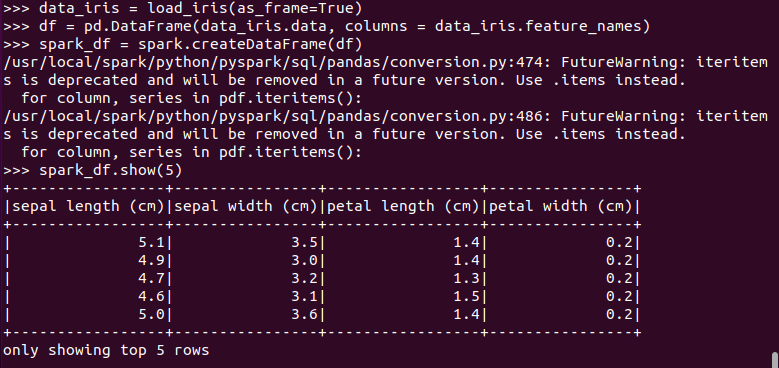
\includegraphics[width=\textwidth]{AdindaAwaliah/grafik 1}
\caption{Grafik pertama }
\label{gam:grafik 1}
\end{figure}

\begin{figure}[!ht]
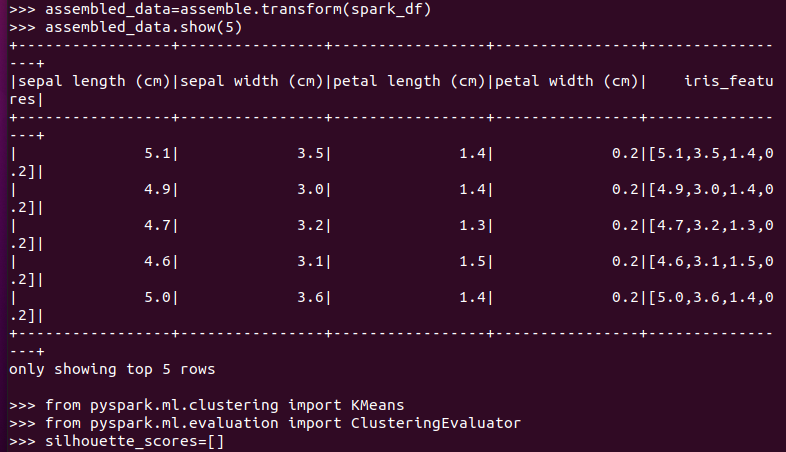
\includegraphics[width=\textwidth]{AdindaAwaliah/grafik 2}
\caption{Grafik kedua }
\label{gam:grafik 2}
\end{figure}

\end{enumerate}